% ********* 中文 ********%%%
% 第4章 设计
\section{Design}

% URN的设计目标是为提供一个统一的RDMA虚拟化框架,以适应混合虚拟化环境,同时实现统一的灵活的RDMA资源管理,并具备与原生RDMA接近的性能。此外,URN应尽可能确保最大的兼容性,对已有RDMA应用透明。
The goals of URN are to provide a unified RDMA virtualization framework for the hybrid virtual environment, meet the unified flexible RDMA resource management and make the performance of virtual RDMA close to the native RDMA meanwhile. Besides, URN should ensure maximum compatibility and be completely transparent to the application. 

%URN主要包含了vRNIC,URN core和mgmt center。vRNIC是对虚拟机和容器通用的虚拟RDMA网卡设备,URN core则是各主机服务器上的用于集中管理RDMA资源的虚拟化层, mgmt center可以跨多主机管理协调RDMA网络的控制策略。在本章,我们介绍了URN中的一些关键性设计工作。
To achieve the above goals, URN mainly consists of the vRNICs, the URN core and the management center. vRNIC is a virtual RDMA network device that is common to virtual machines and containers, URN Core is a virtualization layer for centralized RDMA resource management on each server, and the management center is configured with multiple control policies. In this section, we introduce some key designs in URN.

% 4.1  vRNIC设计
\subsection{vRNIC}

% vRNIC是一个虚拟RDMA设备,由前后端驱动组成。后端在主机端,模拟RDMA设备;前端在guest端, 作为vRNIC的接口,转发guest应用的RDMA 命令到vRNIC后端。
The vRNIC is a virtual RDMA device that consists of a frontend and backend driver. The vRNIC backend is in the host and emulates the RDMA device in the host. As the interface of vRNIC, the vRNIC frontend is in the guest and forwards the RDMA commands from the upper-level RDMA software to the vRNIC backend. 

% 4.1.1 vRNIC后端
\subsubsection{vRNIC Backend}

% vRNIC后端被放在主机用户空间,因为vRNIC后端在用户空间有诸多好处,例如,更小的攻击面,更高的管理灵活性,以及对内核API无依赖等,具体细节可以见2.1节。
The vRNIC backend is placed in the host user-space, because there are many benefits in user-space, which is discussed in detail at section 2.1.

% vRNIC作为一个虚拟RDMA设备,vRNIC后端需要维护关于RDMA网卡的硬件属性,与物理RDMA网卡对应,例如RDMA地址vGID,RDMA设备类型等。此外,在vRNIC的运行过程中,vRNIC后端中需要维护三方面的上下文:
% 1,来自guest的虚拟RDMA上下文信息,主要记录了虚拟RDMA资源的信息;
% 2,由物理网卡创建的RDMA上下文,包含各RDMA资源,由vRNIC后端通过调用verbs库创建和维护;
% 3,虚拟RDMA上下文到物理RDMA上下文之间的对应关系。对应关系是一对一的,因为一对一是RDMA性能隔离的基础。
As a virtual RDMA device, the vRNIC backend needs to maintain the hardware properties that correspond to the physical RNIC, such as the RDMA address GID, the RDMA device vendor, etc. In addition, three aspects of context need to be maintained in the vRNIC backend at the run-time:
(1) Virtual RDMA context information from the guest, mainly including the information about RDMA resources in the guest;
(2) The RDMA context created on the physical RNIC,  including various RDMA resources, which is maintained in the vRNIC backend with the help of the Verbs libraries;
(3) The mapping between the virtual RDMA context and the physical RDMA context. The mapping of RDMA resources is one-to-one, because shared physical RDMA context cannot achieve the performance isolation.

% 如果所有对RDMA资源的操作,均在guest应用和vRNIC后端之间进行拷贝,会引入额外的数据拷贝,导致RDMA性能下降。考虑到控制路径仅涉及到初始化和连接建立的过程,其开销是一次性的,而数据路径包括了RDMA应用的每次数据传输,是影响RDMA性能的关键。因此,为了提高RDMA网络性能,在vRNIC设计过程中,RDMA数据路径中使用了共享内存映射的方式。具体来说,vRNIC后端与guest共享了一块内存区域,vRNIC后端使用该共享内存创建RDMA资源并映射给上层的guest应用,包括MR、QP、CQ和DoorBell等。guest应用基于这些映射的RDMA资源执行数据路径的操作,就是对RDMA物理网卡执行数据操作,不用经过vRNIC后端和虚拟机操作系统,避免了额外的数据拷贝和进程切换的开销,从而实现了与原生RDMA相当的性能。

% 4.1.2 vRNIC前端
\subsubsection{vRNIC Frontend}

% 为了对虚拟机和容器通用,vRNIC前端为不同的虚拟场景提供统一的接口,用于连接guest中的应用和vRNIC后端。虚拟机和容器中有不同的vRNIC前端。 
% 在虚拟机场景中,vRNIC后端是作为虚拟机的外部设备,由虚拟机OS中的vRNIC前端驱动。原生RDMA内核驱动包括与设备无关的OFED模块和设备相关的模块,OFED模块接受来自verbs库的命令,提供了内核层级的RDMA API;设备相关模块调用物理网卡设备的硬件接口,执行来自RDMA命令。对应的,在虚拟机中为了使用vRNIC完成RDMA功能,还需要构建一个自定义的设备相关的驱动模块,实现与原生一样的设备相关接口并注册到OFED模块。与原生RDMA不同的是,在这些接口的逻辑中,OFED中的RDMA命令不会在RDMA网卡硬件上执行,而是被转发到vRNIC前端模块,再由vRNIC后端执行。因此,原生的RDMA应用无需修改便可运行在虚拟机中,而且虚拟机内核空间仍然可以使用RDMA。
% 在容器场景中,vRNIC后端可以和容器应用共享主机操作系统,两者仅位于不同的命名空间。为了在容器的用户空间使用vRNIC,容器的verbs库中与内核RDMA驱动交互的接口,被替换为vRNIC前端接口。Vers库中与内核交互的RDMA命令及参数,被劫持到vRNIC前端,并被转发到vRNIC后端。

% 4.1.3 Guest Verbs库和用户态驱动

% Verbs库基于物理RDMA设备相关的内核及用户态驱动,为RDMA应用提供了Verbs接口。在原生RDMA场景中,Verbs库是面向使用RDMA网卡的应用或其他用户库的通用接口Verbs,在控制路径上,Verbs库接受RDMA应用的Verbs命令并与RDMA内核驱动进行交互,在数据路径上,Verbs库调用设备相关用户态驱动,直接与RDMA物理网卡交互,绕过了操作系统内核。为了让虚拟机或容器中的应用使用vRNIC,同时维持vRNIC对RDMA应用的透明性,虚拟机及容器中的Verbs库在保证与原生接口一致的情况下,需要适配vRNIC架构。

% 在容器中,为了让vRNIC前端接受应用的Verbs命令,将Verbs库中与内核驱动交互的接口替换为与vRNIC前端交互的接口。此外,为了让容器应用与vRNIC后端之间完成RDMA资源的共享内存映射,包括MR、QP/CQ和DoorBell,具体修改如下:
%(1)针对MR:由于MR的内存区域是由应用指定的,在Verbs用户库中将应用指定的MR内存重新映射到指定的共享内存,然后将该共享内存信息随MR命令及参数传递到vRNIC后端。
%(2)针对QP/CQ:原生RDMA中QP/CQ内存的分配是在用户态驱动中进行的,我们在用户态驱动中增加了基于共享内存分配RDMA资源的函数(alloc_shm_buf,参加4.5节),通过该函数分配好QP/CQ内存后,对应的共享内存信息会随RDMA命令和参数传递到vRNIC后端。
% vRNIC后端在收到这些命令和参数后,在创建QP/CQ时,其分配的内存需指定为与虚拟机或容器共享的内存,此时,仍需扩展用户态驱动,主要增加了基于指%定内存地址分配QP/CQ等RDMA资源内存的函数(alloc_assigned_buf,参见4.5节)。

%(3)针对DoorBell:在原生RDMA中,DoorBell由Verbs库打开RDMA内核驱动提供的设备接口并执行映射操作。在vRNIC中,修改了Verbs库中这一操作,让Verbs库打开虚拟的设备接口,将命令和参数传递到主机内核模块执行。

% 在虚拟机中,由于vRNIC在实例化时已经共享了虚拟机的整块物理内存空间,虚拟机应用使用默认的方式分配MR、QP或CQ等RDMA资源的内存,无需对Verbs进行修改。在虚拟机内核的vRNIC前端驱动中,将RDMA资源的内存信息随RDMA命令转发给vRNIC后端,vRNIC后端便可依据这些内存信息,可以创建RDMA资源并映射给虚拟机使用。

% 在完成上述修改后,仍需在虚拟机及容器的设备相关库中对数据路径的工作请求进行额外的地址转换。在数据路径中,guest的RDMA应用往QP中写入工作请求,该请求对应的内存地址是虚拟机或容器应用的地址空间gvm(guest virtual memory),RDMA物理网卡中缓存的MR页表信息则是主机vRNIC后端共享MR的地址空间s-hvm(shared host virtual memory),因此,仍然需要对RDMA工作请求中的gvm进行转换,将gvm转换成s-hvm,再将转换地址后的工作请求写入已经映射的QP中,之后物理RDMA网卡才可以执行guest的工作请求。对于这一地址转换工作,需要修改guest中的 用户态驱动。具体做法是,在guest用户态驱动中记录有MR资源的地址映射关系,包括MR的Key,gvm,s-hvm,即{key, gvm, s-hvm},待guest应用执行数据操作时,根据key查询映射关系,将对应的gvm转换成s-hvm即可。

% 基于上述修改,无论是虚拟机还是容器,RDMA应用在控制路径中,RDMA命令经过Verbs库,vRNIC前端到达vRNIC后端,在vRNIC后端中创建RDMA源时会确保资源映射到guest应用。基于映射的RDMA资源,数据路径不需要经过虚拟机操作系统和vRNIC后端,RDMA工作请求直接在guest本地驱动物理RDMA网卡执行,避免了数据路径频繁的拷贝或切换开销。

% 4.2  URN Core 设计
\subsection{URN Core}

% 为了对vRNIC进行统一管理,高效利用物理RDMA网卡,我们构建了一个统一的虚拟层URN core。URN core部署于集群的每台服务器上,其主要功能包括实例化vRNIC和配置虚拟RDMA网络等。

% 4.2.1 实例化vRNIC 
% URN core在收到虚拟机或容器应用申请vRNIC的请求后,会实例化vRNIC。URN core在实例化vRNIC的主要工作包括: 初始化vRNIC属性、绑定vRNIC到物理网卡、构建vRNIC前后端消息通道以及隔离各vRNIC实例等。

% 初始化vRNIC属性:为了让vRNIC具备与硬件一致的功能接口,URN Core需要对vRNIC的不变属性进行初始化。vRNIC中的不变属性包括RDMA地址vGID,设备号等等。对于RDMA地址vGID,URN core会随机生成IPv6格式的虚拟值,同时通过mgmt center进行协调和登记,以确保各vRNIC的RDMA地址等信息是不冲突的并维护在统一的数据库中。

% 绑定vRNIC到物理网卡:vRNIC实例需要依靠物理网卡实现RDMA功能,因此,实例化vRNIC时需要将vRNIC实例与对应的物理RDMA网卡绑定。如果是多网卡设备或者多个网卡接口(如使用SR-IOV),还需确定从vRNIC到对应物理网卡接口的映射关系。

% 构建vRNIC消息通道:URN Core需要构建vRNIC后端与vRNIC前端(guest)之间的消息通道。对于容器来说,容器与vRNIC后端共享某一IPC命名空间,即可完成vRNIC前端与后端之间的消息交互。对于虚拟机来说,由于vRNIC后端在主机用户空间,而hypervisor位于主机内核空间。为了避免guest的消息先拷贝到hypervisor层再到vRNIC后端,我们在vRNIC后端与guest中的vRNIC前端之间构建一块共享内存,以此作为消息通道。具体来说,虚拟机内存区域对应的物理页面,与vRNIC后端之间是共享的。这样,guest中的任意RDMA消息,均可以直接由vRNIC后端获取,而无需进入到主机内核空间,同时也减少了消息从guest到vRNIC后端的延迟。

% vRNIC实例隔离:URN core需要确保各vRNIC之间的消息通道是隔离的。在云环境中,同一主机上可能部署多个虚拟机或容器,该主机的URN core需要实例化多个vRNIC后端,以满足不同的guest实例。因此,需要确保各vRNIC之间的消息通道是隔离的,尤其是容器,由于其隔离性不如虚拟机彻底。如果多个容器和主机共享同一文件命名空间或IPC空间,那么,很容易通过扫描获取到其他容器或虚拟机vRNIC的消息通道。URN core利用了文件命名空间的机制,文件命名空间中的文件对于其他命名空间是不可见的。URN core在实例化vRNIC时,将各vRNIC消息通道对应的文件位于不同的命名空间,从而实现了各vRNIC实例之间消息通道的隔离。

% 4.2.2 配置虚拟RDMA网络

% URN core在实例化vRNIC后,需要对vRNIC的网络进行配置,包括虚拟RDMA地址配置以及虚拟RDMA路由配置。

% 对于虚拟RDMA地址配置,URN core 在实例化vRNIC时, 给vRNIC配置的vGID是虚拟值,与物理网卡的GID无关。

% 对于虚拟RDMA路由配置,每台主机的URN core中配置了虚拟RDMA网络路由规则。具体来说,URN core在实例化vRNIC时,还给每个vRNIC都配置了组ID,路由规则的定义形式为:{group ID1, group ID2, Policy}。例如,如图4所示,容器1和容器2的vrnic被配置到同一组中,因此允许创建RDMA连接。作为对比,容器1和虚拟机1属于不同的用户组,按路由规则无法建立RDMA连接。各虚拟实例之间建立RDMA连接的具体细节可以参考4.3.1。

% RDMA网络与传统TCP不同,RDMA还支持单边操作。在guest应用的RDMA单边操作中,RDMA的工作请求中包含了远端guest MR的内存地址及key,远端MR内存地址同样需要在RDMA用户态驱动中完成转换,将远端的gvm转换为远端vRNIC后端的s-hvm。为了便于guest应用查询远端gvm对应的s-hvm,我们在URN core中建立了一个分布式的KV数据库,存储各节点注册MR的映射关系{key,gvm,s-hvm}。在guest应用执行单边操作时,将向URN core 中的分布式KV数据库查询,以获取远端对应的s-hvm,缓存到本地并写入工作请求。

% 总之,URN core中的虚拟网络配置是动态调整的,因此,容器和虚拟机迁移后无需更改物理网卡及交换机等硬件的网络配置,实现便携的虚拟机或容器迁移。基于URN core中的路由规则,可以支持云环境中的多租户隔离。而各URN core存储的MR地址映射关系,对RDMA网络特有的单边操作给予了支持。


\begin{figure}[!ht]
	\centering
	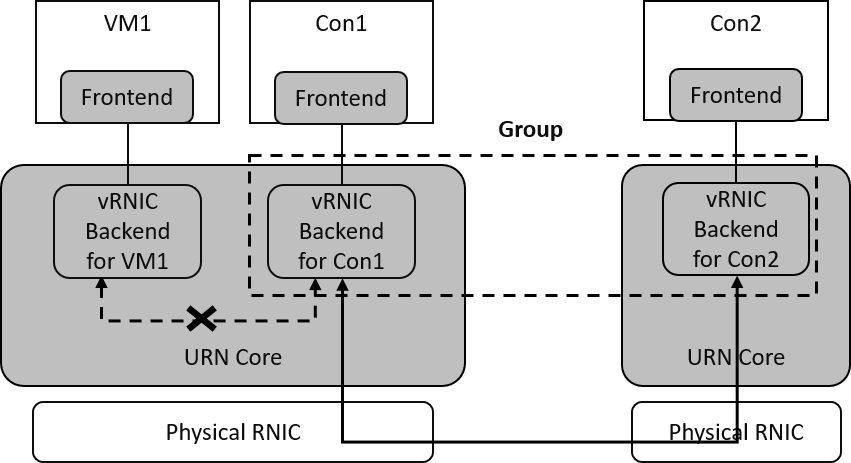
\includegraphics[width=1.0\linewidth]{images/route-config}
	\caption{Group Configuration and Routing: The vRNICs of container 1 and container 2 are configured in one group. Thus, two containers can create RDMA connections. And VM 1 are not allowed to create RDMA connections to containers in this figure because it is not added into the group. }
	\label{fig:route-config}
\end{figure}


% 4.3 虚拟RDMA workflow
\subsection{Virtual RDMA Workflow}
% 为了更好地说明虚拟RDMA的工作过程,我们介绍了虚拟RDMA的详细工作流程,如图4所示。虚拟RDMA的工作流程涉及guest中的应用、verbs库以及主机的vRNIC后端交互。整个工作流程依次分为初始化阶段、连接阶段和数据阶段。其中,初始化阶段和连接阶段属于RDMA控制路径,初始化阶段分别包括设备打开和RDMA资源创建,连接阶段中RDMA应用与远端建立连接。数据阶段中RDMA应用执行数据路径的传输操作。

\begin{figure}[!ht]
	\centering
	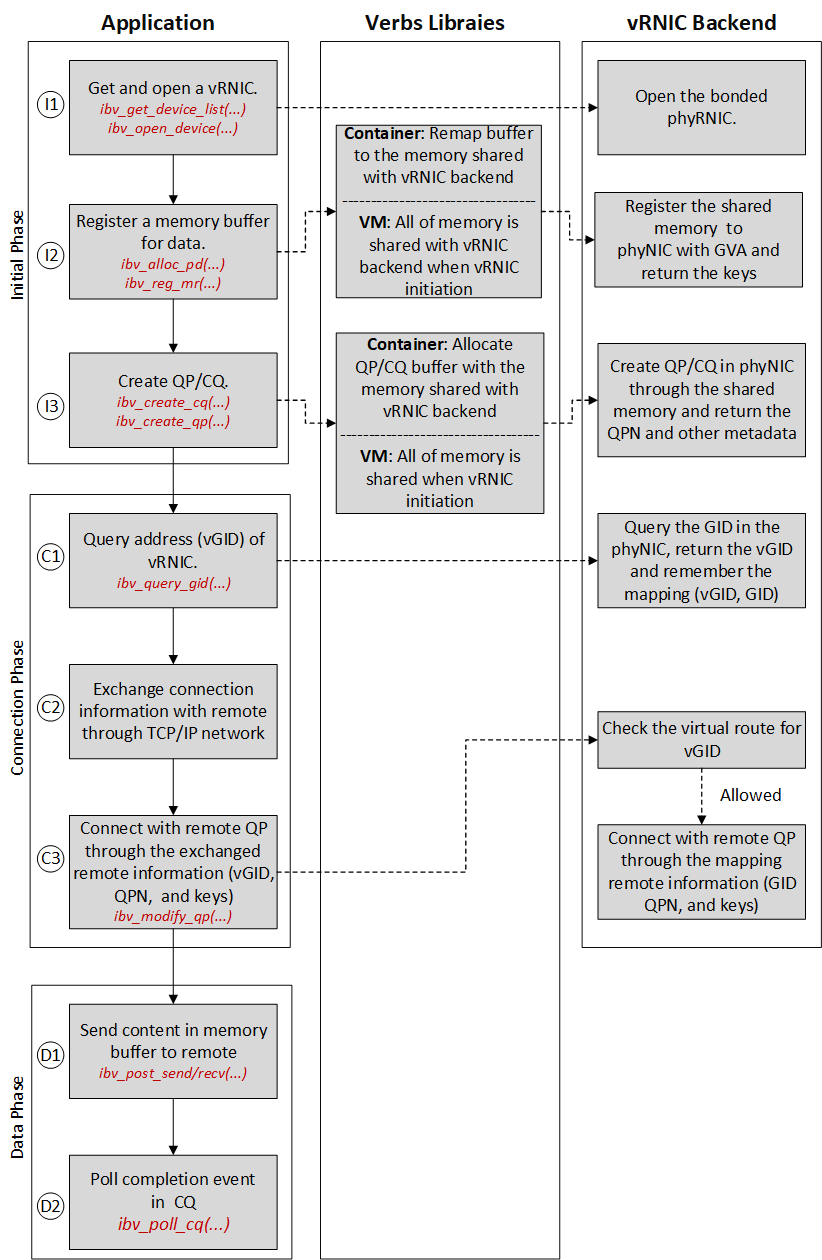
\includegraphics[width=1\linewidth]{images/RDMA-path.png}
	\caption{The Workflow of RDMA SEND operation}
	\label{fig:route-config}
\end{figure}

% 4.3.1 初始化阶段
%  初始化阶段主要完成资源的初始化,分别包括设备打开(I1)、注册内存buffer(I2)和创建QP/CQ等RDMA资源(I3)。具体细节如下: 

% I1(Guest应用打开vRNIC设备):Guest应用依次调用Verbs接口ibv_get_devicelist和ibv_open_device,获取并打开vRNIC设备。 Guest中的Verbs库将传递这些命令和参数到vRNIC后端,vRNIC后端会打开在vRNIC实例化时绑定的物理RDMA设备。

% I2(Guest应用注册MR):在容器中,Verbs库中将应用指定的MR内存重新映射到某一共享内存,然后将该路径随MR命令及参数传递到vRNIC后端,虚拟机无需此步骤,因为在实例化vRNIC时已与vRNIC后端共享整个内存。对于容器和虚拟机,vRNIC后端在收到该命令及参数后,会使用对应的共享内存注册MR,并返回MR内存地址(s-hvm)和key等信息,在虚拟机和容器的Verbs库中,则会记录guest中MR内存地址(gvm)与s-hvm,以及MR的key,这三者的对应关系,用于后续的数据路径操作。

% I3(Guest应用创建QP/CQ):在容器中,Verbs及其设备相关库使用共享内存分配QP/CQ的buffer,对应的共享内存路径会随RDMA命令和参数传递到vRNIC后端,虚拟机无需此步骤,因为在实例化vRNIC时已与vRNIC后端共享整个内存。对于容器和虚拟机,vRNIC后端在收到这些命令和参数后,在创建QP/CQ时,使用接收的共享内存地址分配QP/CQ等RDMA资源内存,在创建资源后,vRNIC后端会返回QPN等RDMA资源的元数据。 

%4.3.2 连接阶段
% 连接阶段主要建立基于QP的RDMA连接,依次包括查询GID(C1)、交换连接信息(C2)和基于QP建立连接(C3),具体细节如下:

% C1(获取GID):Guest应用执行ibv_query_gid,请求获取vRNIC的vGID地址,vRNIC后端在收到该命令后,会获取绑定的物理RDMA网卡的GID,并记录(vGID,GID)对应关系。不过,vRNIC后端返回给guest的仍然是vGID。

% C2(交换连接信息):Guest应用与远端RDMA连接所需的地址信息vGID,QPN和MR key等。 该步骤完全由应用程序完成,无需依靠Verbs库和vRNIC后端。例如,应用中可以使用TCP socket来与远端guest应用完成这一系列信息的交换。

% C3(基于QP建立连接):Guest应用将C2获取的远端vGID、QPN等信息作为ibv_modify_qp的参数,基于QP与远端建立RDMA连接。该命令转发到vRNIC后端后,vRNIC后端会先根据设置的路由表规则进行判断,如果远端vGID符合路由规则,就会将vGID转换成对应的GID,基于GID,QP ID及Key完成与远端vRNIC后端QP的配对。从vGID到GID的转换,实现了RDMA连接的网络虚拟化。

% 4.3.3 数据阶段
% 数据路径发生在连接建立后,对注册的MR中的内容执行操作。RDMA的数据路径包括图中的D1和D2。

% D1(收发数据):Guest应用发送或接收MR中的数据。由于MR和QP已经完成了资源映射,此时,数据操作时的数据块(MR中)和工作请求(QPs)可以直接由RDMA物理网卡访问。不过,工作请求中的地址信息仍然是guest中的地址,而第三步中创建MR时,物理网卡记录是vRNIC后端中的页表信息。因此,需要借助前面缓存的三元组信息,将工作请求中的guest地址转换为vRNIC后端地址,再填充到QP中。如果是单边操作,其工作请求中还包含远端地址信息,在第一次执行命令时还需要向vRNIC后端发送请求,获取URN core中存储的远端MR地址映射关系,并缓存到本地。然后将工作请求中的本地及远端地址均进行转换,填充到QP中。

% D2(轮询CQ):Guest应用轮询CQ获取数据操作的完成事件。由于CQ已经完成了资源映射,此时,物理网卡中工作完成的通知会直接写入到guest的CQ中。


% 4.4 mgmt center
\subsection{Management Center}

% 在URN框架里,整个集群配备一个mgmt center,作为配置管理策略,存储各节点RDMA资源信息的中心。

% 通过mgmt center,管理者向不同节点的URN core下发各种策略,包括控制平面策略,如连接管理,防火墙等;和数据平面策略,如Qos、流量计费等。管理框架图如图5所示:策略由mgmt center下发到URN core,URN core通过agent接收策略后,其中,URN core将控制平面策略配置给管理的各vRNIC后端。对于数据平面策略,URN core将其发送给各guest Verbs库中的agent,然后在各RDMA应用本地执行。

%  连接管理、防火墙等控制平面策略主要基于RDMA连接进行,而RDMA连接依靠QP等RDMA资源,因此,这些策略主要依靠RDMA资源,如QP进行控制。由于包括QP在内的所有RDMA资源均已经映射在vRNIC后端中,因此,控制策略可以直接传送到各vRNIC后端,依靠映射的RDMA资源执行。 对于数据路径,依靠监控各vRNIC后端维护的映射好的RDMA资源,如QP/CQ等,可以完成QoS等数据功能。然而,这样做将消耗额外的CPU资源而且对轮询的处理效率要求极高。因此,本文将数据策略进一步从URN core下发到各guest的用户库,在各RDMA应用本地执行,策略执行结果则可以返回给URN core或mgmt center。注意,这些扩展需要所有客户机都信任库,并且这些修改应该包含在TCB(可信计算库)中。对照native的RDMA,其数据路径绕过了操作系统内核,而RDMA物理网卡的数据管理功能及其有限,因此,其细粒度的数据管理同样需要由Verbs库配合执行。

\begin{figure}[!ht]
	\centering
	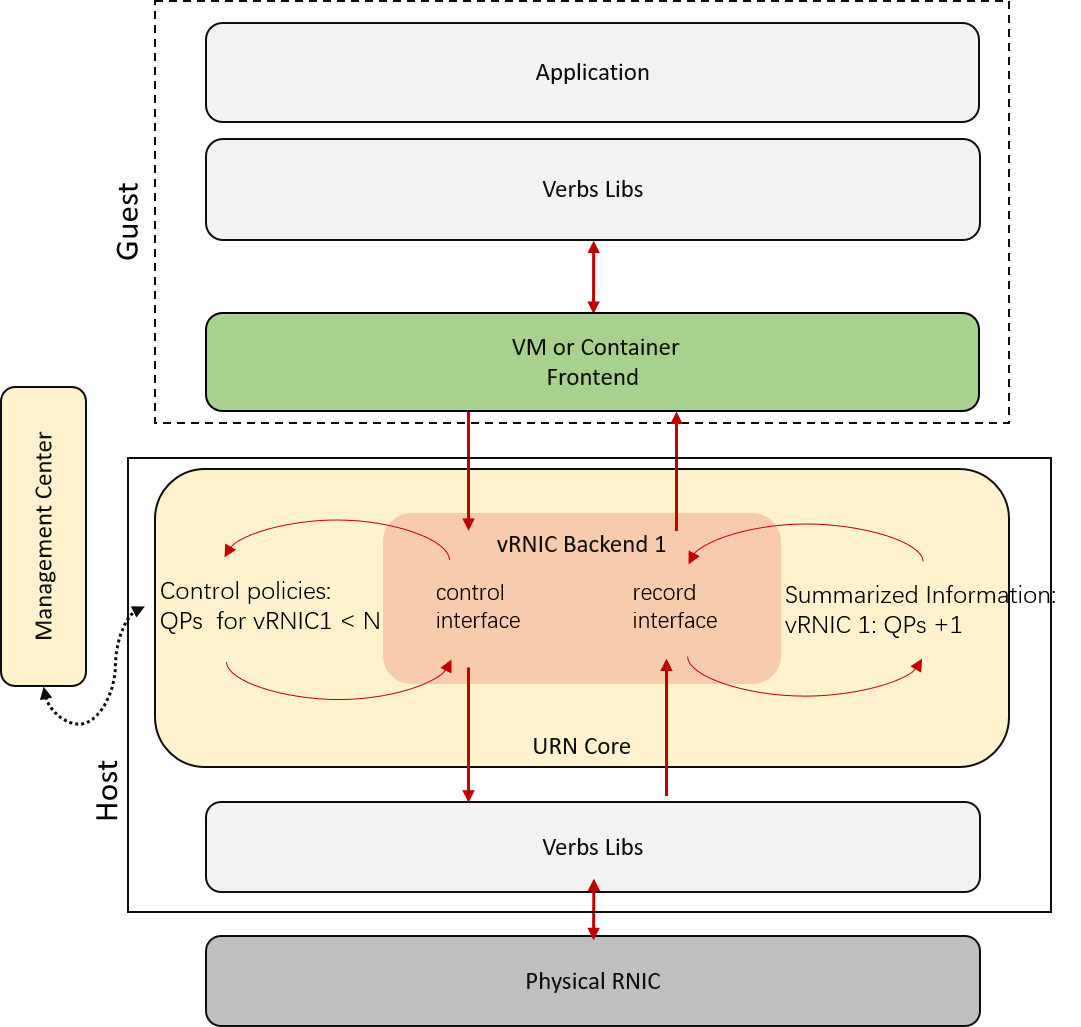
\includegraphics[width=1\linewidth]{images/urn-interface.png}
	\caption{The Architecture of URN Management}
	\label{fig:route-config}
\end{figure}

% 4.5 discussion
% 随着云计算环境的复杂化,不同的需求越来越多,对RDMA虚拟化提出了更多的要求。结合可能的需求,本节讨论了RDMA虚拟化可能面临的一些需求和解决思路:
\subsection{Discussion}

%  (1)虚拟机迁移: 容器或虚拟机迁移在云中有很多好处,例如资源利用和故障转移。迁移分为脱机迁移和动态迁移。在脱机迁移中,虚拟机或容器关机后,迁移到远端后重新启动。因为URN core维护了网络地址的映射关系,该关系可以直接发送给迁移后节点的URN core,无需修改guest 中RDMA应用内部的网络地址。对于动态迁移,一般都需要借助AccelNet方案【引用】,应用释放RDMA资源,使用TCP/IP网络完成迁移,然后显式地重新建立RDMA连接。对于这种方式,我们也可以无缝支持。
 Virtual Instances Migration: Migration of containers or VMs has many benefits in clouds, e.g. resource utilization and fail-over. With the virtual RDMA network, URN can support offline migration without reconfiguring the physical RDMA network for applications. In specific, after rebooting the migrated virtual instance, the application can rebuild the RDMA connection through the same network address. The only work is modifying the address mapping in URN core. Currently, for live migrations, it is still hard because memory regions in RDMA application may be uncertain under bypassing or one-side communication. And the problem is unrelated to URN.
 
 % (2)对RDMA虚拟化扩展的支持:RDMA虚拟化中,需要对QP/CQ等RDMA资源进行资源映射,避免额外的数据拷贝及切换开销。现有的Verbs库和用户态驱动没有对RDMA资源映射的支持。为此,我们建议Verbs库或设备相关库中增加以下API,以加强对各场景下RDMA虚拟化的支持,尤其是应用可以使用新增加的Verbs接口显式地完成MR、QP/CQ等资源的映射。如下表所示:
% API  所属库  功能 
% alloc_shm_buf()  设备相关库 创建并分组共享内存作为RDMA资源内存
% alloc_assigned_buf(addr, size) 设备相关库 为RDMA资源指定某一内存区域
% ibv_create_shm_qp/cq() 基于共享内存区域创建QP/CQ
% ibv_assigned_qp/cq 使用指定的内存区域创建QP/CQ
% ibv_reg_shm_mr() 使用共享内存区域注册MR

% 此外,为了实现高性能的数据传输,RDMA网卡缓存了应用注册内存的页表信息。在用户态虚拟化后,现有的RDMA网卡只能缓存虚拟层MR的页表信息,而无法缓存guest应用使用MR的页表信息。在URN的实现里面,尽管通过在URN core KV数据库和本地缓存数据库实现了高效的地址转换,但是引入了额外的工作量。因此,为了更好地适配虚拟化场景,建议Verbs库在创建MR时额外提供一个指定网卡缓存guest应用页表的地址参数,如原来的ibv_reg_mr(..., s-hva)扩展为ibv_reg_mr(..., s-hva, gva)。稍后,RDMA内核驱动可以根据新注入的gva参数,为该MR指定与guest应用对应的页表。

% (3)扩展虚拟Verbs接口: 目前我们设计Verbs库的主要考虑是与原生的Verbs库兼容,以实现对RDMA应用的透明性,但是,这样会导致容器应用只能基于URN verbs库使用虚拟RDMA,或者基于原生Verbs库使用RDMA,从而导致了使用RDMA的局限性。解决这一问题的可能思路是,扩展Verbs库,增加获取虚拟RDMA设备的专有Verbs接口,供应用选择调用。
%%%*********************%%%
